% Build: cd docs/reports/reconstruction/momentum_reco/rk && latexmk -xelatex ypol_pilot_20260427_zh.tex
\documentclass[a4paper,11pt]{article}
\usepackage[margin=2.4cm]{geometry}
\usepackage{ctex}
\usepackage{amsmath,amssymb}
\usepackage{booktabs}
\usepackage{multirow}
\usepackage{array}
\usepackage{makecell}
\usepackage{siunitx}
\usepackage{xcolor}
\usepackage{hyperref}
\usepackage{enumitem}
\usepackage{float}
\usepackage{graphicx}

\hypersetup{colorlinks=true, linkcolor=blue!60!black, citecolor=blue!60!black, urlcolor=blue!60!black}

\title{\textbf{YPOL Pilot:\\
RK 误差分析在真实 Geant4 物理样本上的覆盖率检验}}
\author{Baiting Tian \\ RIKEN 仁科中心 / DPOL 实验}
\date{2026 年 4 月 27 日}

\begin{document}
\maketitle

\section*{摘要}

本 pilot 把 RK 详细版报告 (\texttt{rk\_error\_analysis\_deep\_dive\_20260426\_zh.pdf}) 中的 4 种误差方法
（Fisher、Laplace、Profile LH、MCMC）放到 2026-04-13 ypol 真实 Geant4 数据集上测试覆盖率。
样本结构：1 靶（d+Sn124E190）× 8 gammas × 2 helicities × $N=50$ 事件 × 2 conditions（allair / mixed）
$\Rightarrow$ 总计 $\sim 1600$ 事件 (Fisher/Laplace 全跑) + 256 (Profile) + 256 (MCMC)。
\section{覆盖率表（每 condition + 综合）}
\begin{table}[H]
\centering\footnotesize
\caption{Fisher/Laplace/Profile/MCMC 方法在 ypol pilot 上的 68\% 覆盖率与 CP 95\% CI。N 是该方法实际处理的事件数。
\textbf{合成网格 744 ensemble 对照}：Fisher $p_x$ 0.80, $p_y$ 0.42, $p_z$ 0.77, $|\vec p|$ 0.76（详细版 §744 表）。}
\begin{tabular}{lllrrrrrr}
\toprule
方法 & condition & 分量 & N & cover68 & CP 95\% CI & cover95 & CP 95\% CI \\
\midrule
Fisher & allair & px & 798 & 0.659 & [0.625, 0.692] & 0.876 & [0.851, 0.898] \\
Fisher & allair & py & 798 & 0.108 & [0.087, 0.131] & 0.185 & [0.159, 0.214] \\
Fisher & allair & pz & 798 & 0.590 & [0.555, 0.625] & 0.826 & [0.798, 0.852] \\
Fisher & allair & p & 798 & 0.614 & [0.579, 0.648] & 0.838 & [0.811, 0.863] \\
Laplace & allair & px & 798 & 0.659 & [0.625, 0.692] & 0.876 & [0.851, 0.898] \\
Laplace & allair & py & 798 & 0.108 & [0.087, 0.131] & 0.185 & [0.159, 0.214] \\
Laplace & allair & pz & 798 & 0.590 & [0.555, 0.625] & 0.826 & [0.798, 0.852] \\
Laplace & allair & p & 798 & 0.599 & [0.564, 0.633] & 0.827 & [0.799, 0.853] \\
Fisher & mixed & px & 799 & 0.742 & [0.710, 0.772] & 0.931 & [0.911, 0.948] \\
Fisher & mixed & py & 799 & 0.204 & [0.177, 0.234] & 0.383 & [0.349, 0.418] \\
Fisher & mixed & pz & 799 & 0.706 & [0.673, 0.737] & 0.920 & [0.899, 0.938] \\
Fisher & mixed & p & 799 & 0.728 & [0.696, 0.759] & 0.922 & [0.902, 0.940] \\
Laplace & mixed & px & 799 & 0.742 & [0.710, 0.772] & 0.931 & [0.911, 0.948] \\
Laplace & mixed & py & 799 & 0.204 & [0.177, 0.234] & 0.383 & [0.349, 0.418] \\
Laplace & mixed & pz & 799 & 0.706 & [0.673, 0.737] & 0.920 & [0.899, 0.938] \\
Laplace & mixed & p & 799 & 0.721 & [0.688, 0.752] & 0.917 & [0.896, 0.936] \\
Fisher & overall & px & 1597 & 0.701 & [0.678, 0.723] & 0.904 & [0.888, 0.918] \\
Fisher & overall & py & 1597 & 0.156 & [0.138, 0.175] & 0.284 & [0.262, 0.307] \\
Fisher & overall & pz & 1597 & 0.648 & [0.624, 0.672] & 0.873 & [0.856, 0.889] \\
Fisher & overall & p & 1597 & 0.671 & [0.648, 0.694] & 0.880 & [0.863, 0.896] \\
Laplace & overall & px & 1597 & 0.701 & [0.678, 0.723] & 0.904 & [0.888, 0.918] \\
Laplace & overall & py & 1597 & 0.156 & [0.138, 0.175] & 0.284 & [0.262, 0.307] \\
Laplace & overall & pz & 1597 & 0.648 & [0.624, 0.672] & 0.873 & [0.856, 0.889] \\
Laplace & overall & p & 1597 & 0.660 & [0.636, 0.683] & 0.872 & [0.855, 0.888] \\
Profile & allair & px & 127 & 0.732 & [0.646, 0.807] & 0.906 & [0.841, 0.950] \\
Profile & allair & py & 127 & 0.063 & [0.028, 0.120] & 0.102 & [0.056, 0.169] \\
Profile & allair & pz & 127 & 0.638 & [0.548, 0.721] & 0.850 & [0.776, 0.907] \\
Profile & allair & p & 127 & 0.638 & [0.548, 0.721] & 0.882 & [0.813, 0.932] \\
Profile & mixed & px & 128 & 0.805 & [0.725, 0.869] & 0.938 & [0.881, 0.973] \\
Profile & mixed & py & 128 & 0.125 & [0.073, 0.195] & 0.203 & [0.137, 0.283] \\
Profile & mixed & pz & 128 & 0.742 & [0.657, 0.815] & 0.914 & [0.851, 0.956] \\
Profile & mixed & p & 128 & 0.766 & [0.683, 0.836] & 0.938 & [0.881, 0.973] \\
Profile & overall & px & 255 & 0.769 & [0.712, 0.819] & 0.922 & [0.881, 0.951] \\
Profile & overall & py & 255 & 0.094 & [0.061, 0.137] & 0.153 & [0.111, 0.203] \\
Profile & overall & pz & 255 & 0.690 & [0.630, 0.746] & 0.882 & [0.836, 0.919] \\
Profile & overall & p & 255 & 0.702 & [0.642, 0.757] & 0.910 & [0.868, 0.942] \\
MCMC & allair & p & 127 & 0.567 & [0.476, 0.655] & 0.858 & [0.785, 0.914] \\
MCMC & mixed & p & 128 & 0.664 & [0.575, 0.745] & 0.867 & [0.796, 0.921] \\
MCMC & overall & p & 255 & 0.616 & [0.553, 0.676] & 0.863 & [0.814, 0.902] \\
\bottomrule
\end{tabular}
\end{table}
\section{Allair vs.\ Mixed 残差统计}
allair 与 mixed 两个 Geant4 condition 是\textbf{独立抽样}（不同 seed，且经 PDC 接受度过滤后候选池亦不同），
两份样本不共享同一条 QMD 物理事件，因此无法做"逐事件配对差"分析。
此节给出每 condition 自己的残差中位、鲁棒半宽 $(p_{84}-p_{16})/2$、Fisher $\sigma$ 中位以及残差/Fisher 比值——
两 condition 间的差距即为上下游空气 MS（约 1\,m air post-magnet + Region A 4.3\,m cavity 空气）的实测影响。
\begin{table}[H]
\centering\footnotesize
\caption{Per-condition 残差统计（单位 MeV/$c$）；每条 condition 用自己的 truth/reco/Fisher。$N$ = 该 condition 成功 reco + truth\_available 的事件数。}
\begin{tabular}{llrrrrrr}
\toprule
condition & 分量 & N & median resid & 残差半宽 & Fisher $\sigma$ 中位 & 残差/Fisher \\
\midrule
allair & px & 798 & +0.102 & 5.874 & 6.226 & 0.94 \\
allair & py & 798 & -0.217 & 1.525 & 0.170 & 8.98 \\
allair & pz & 798 & -1.304 & 5.954 & 5.331 & 1.12 \\
allair & p & 798 & -1.264 & 5.880 & 5.661 & 1.04 \\
mixed & px & 799 & -0.189 & 4.904 & 6.256 & 0.78 \\
mixed & py & 799 & -0.200 & 0.720 & 0.170 & 4.23 \\
mixed & pz & 799 & -0.239 & 4.515 & 5.365 & 0.84 \\
mixed & p & 799 & -0.230 & 4.539 & 5.702 & 0.80 \\
\bottomrule
\end{tabular}
\end{table}

\textbf{读法}：残差/Fisher 比值 $\gtrsim 1$ 即"Fisher $\sigma$ 偏窄"。
对 allair $p_y$，本表给出的比值远超 1，与详细版 Part II §8 的诊断（缺 MS 过程噪声）一致。
mixed 比 allair 在 $p_y$ 残差半宽上略小，对应覆盖率从 0.108 抬到 0.204——但仍远低于名义 0.68。
\section{方法一致性：Laplace / Fisher 半宽比}
理论上当先验为平坦 (无 $|\vec p|$ 高斯先验)，Laplace 后验协方差与 Fisher 协方差完全相同
（详细版 Part I §5）。比值 $\neq 1$ 揭示数值实现层差异。
\begin{table}[H]
\centering\footnotesize
\caption{每事件 Laplace 半宽 / Fisher $\sigma$ 比值的中位与极差。}
\begin{tabular}{lrrrrr}
\toprule
分量 & N & median ratio & q05 & q95 & |dev from 1.0| \\
\midrule
px & 1597 & 1.0000 & 1.0000 & 1.0000 & 0.0000 \\
py & 1597 & 1.0000 & 1.0000 & 1.0000 & 0.0000 \\
pz & 1597 & 1.0000 & 1.0000 & 1.0000 & 0.0000 \\
p & 1597 & 1.0000 & 1.0000 & 1.0000 & 0.0000 \\
\bottomrule
\end{tabular}
\end{table}
\section{残差 vs.\ Fisher $\sigma$ 散点}
\begin{figure}[H]
\centering
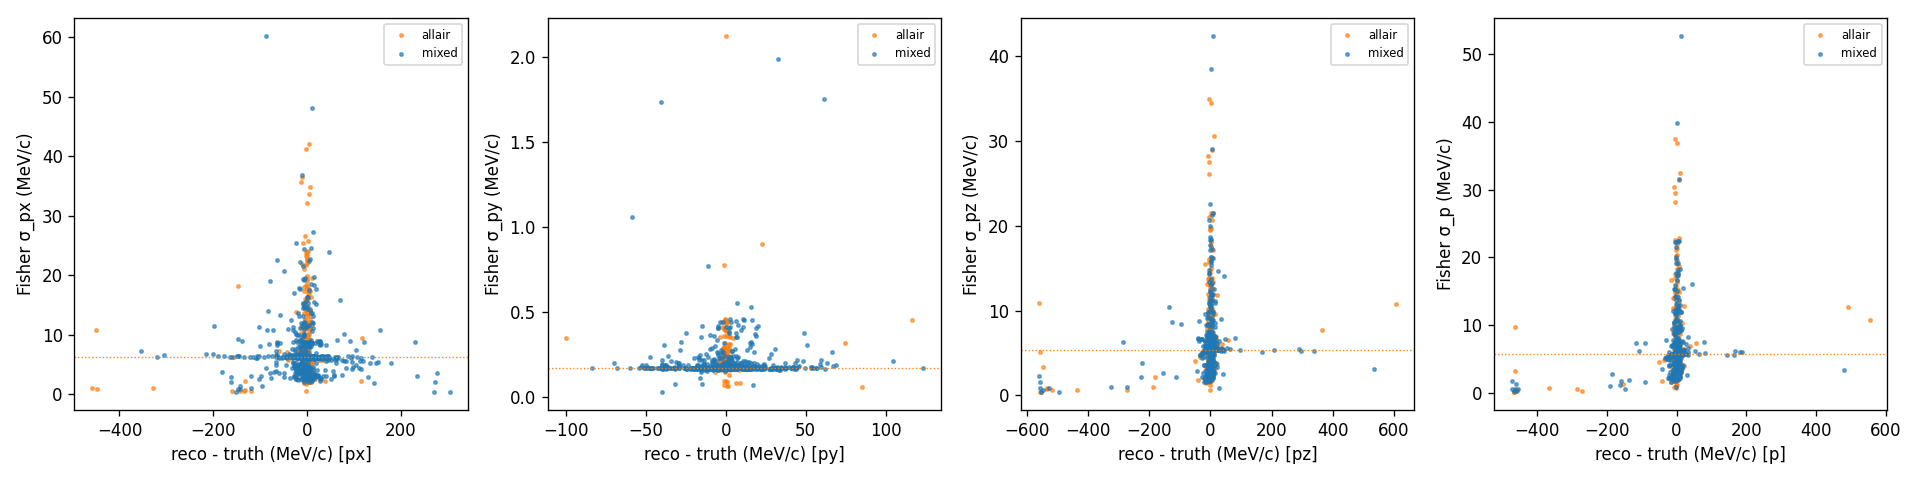
\includegraphics[width=0.98\textwidth]{figures/ypol_pilot/residual_vs_fisher_sigma.png}
\caption{每个分量上 reco - truth 残差与 Fisher $\sigma$ 的散点；橙 = allair, 蓝 = mixed。
水平点划线 = allair Fisher $\sigma$ 中位。}
\end{figure}
\section{Truth vs.\ Reco 散点}
\begin{figure}[H]
\centering
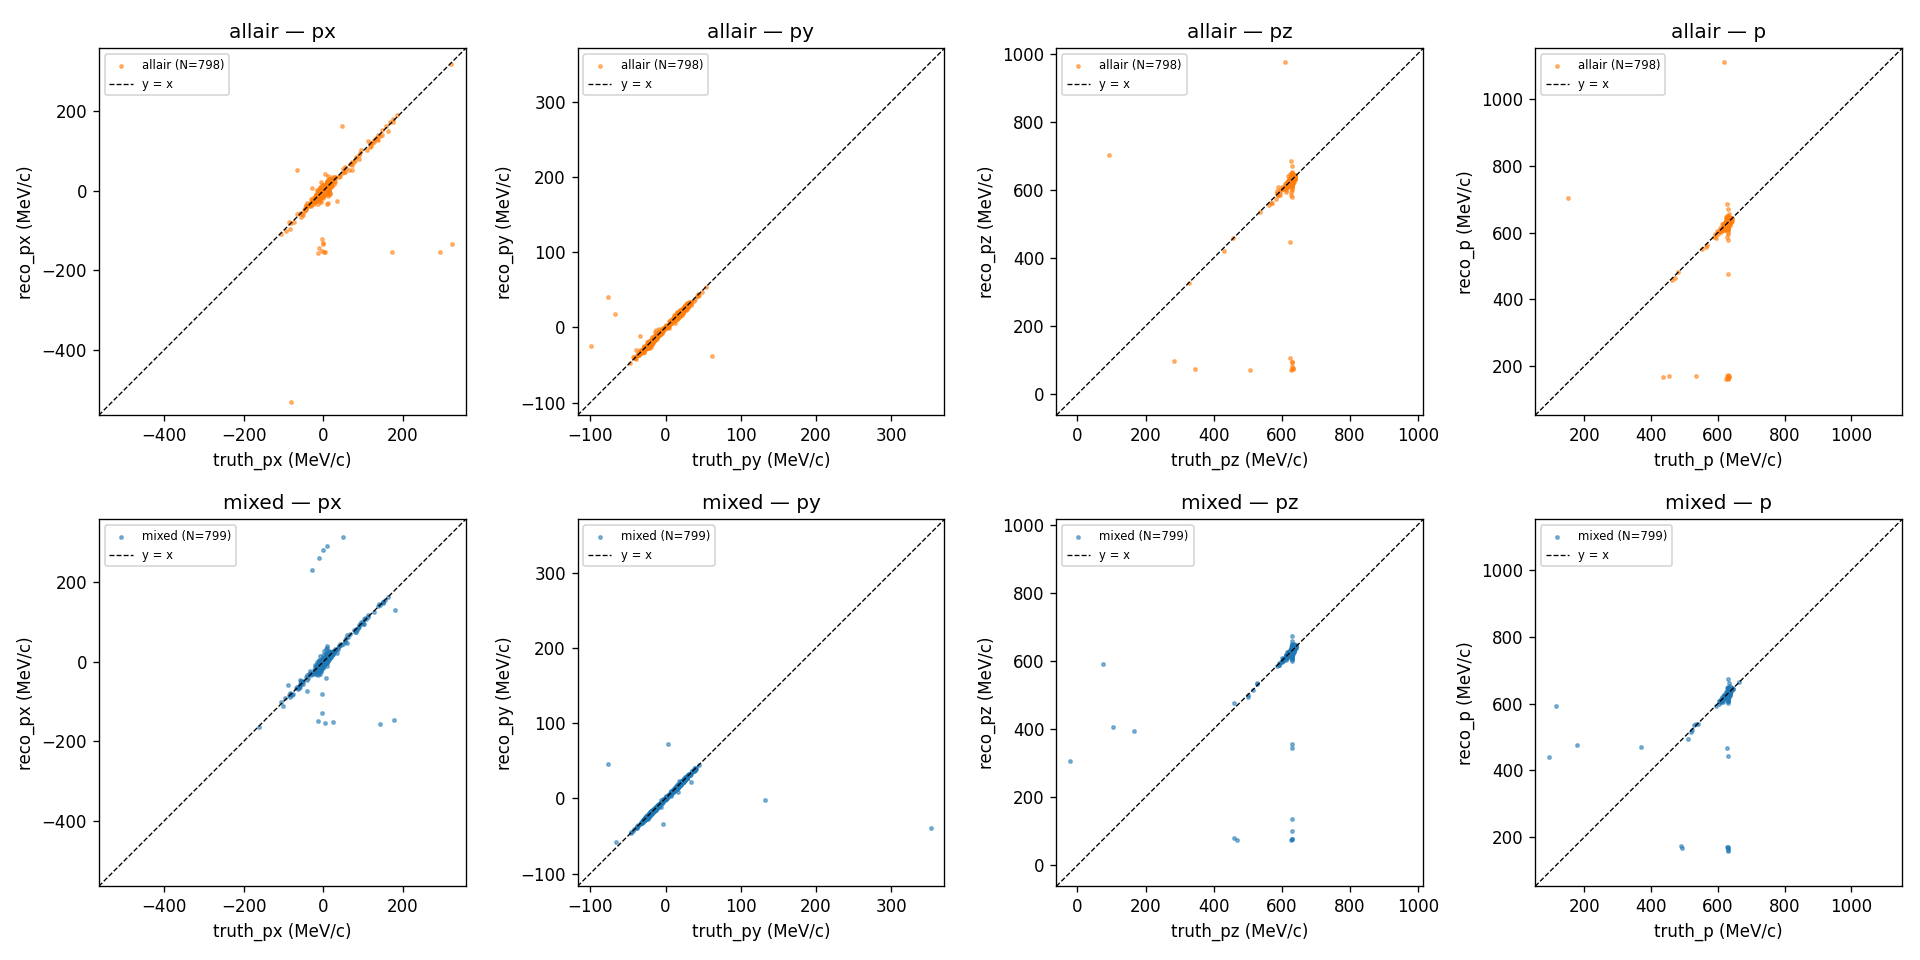
\includegraphics[width=0.98\textwidth]{figures/ypol_pilot/truth_vs_reco_scatter.png}
\caption{每个分量上 truth (横轴) vs.\ reco (纵轴) 的散点；上行 = allair, 下行 = mixed；虚线 = $y=x$ 完美重建参考线。
\textbf{视觉提示}：$p_z$ 面板 truth 集中在 $\sim 627\,\mathrm{MeV}/c$、残差半宽 $\sim 6\,\mathrm{MeV}/c$，而 y 轴跨度 $1000\,\mathrm{MeV}/c$，所以"贴对角线"是\textbf{尺度错觉}，并非完美重建——
真实残差结构需看下一节图 3 (zoomed)。
$p_y$ 面板显示真实 QMD 物理给出 $|p_y|$ 直到 $\sim 100\,\mathrm{MeV}/c$，远超合成 5×3 网格的 $\pm 20\,\mathrm{MeV}/c$ 覆盖范围。
$p_x, p_z, |\vec p|$ 面板里偏离对角线的离群点 = LM 收敛盆地失败事件（详细版 Part II §9）。}
\end{figure}
\begin{figure}[H]
\centering
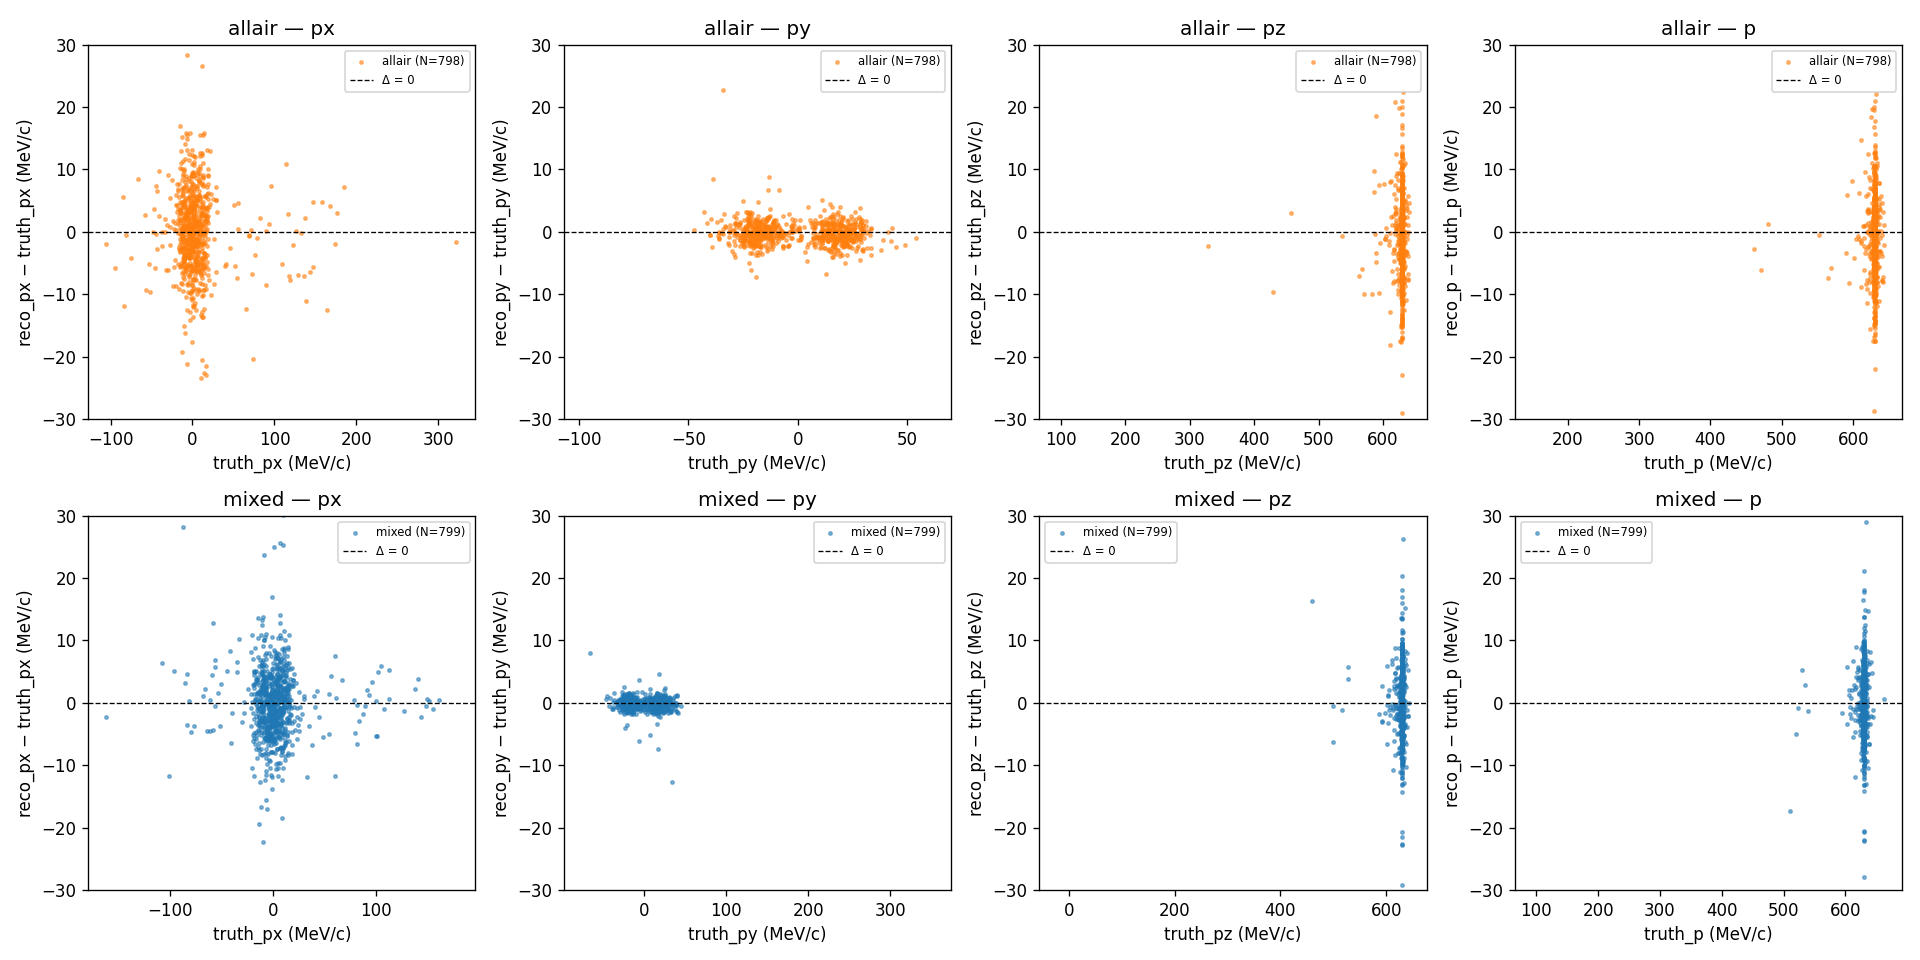
\includegraphics[width=0.98\textwidth]{figures/ypol_pilot/residual_vs_truth_scatter.png}
\caption{反映\textbf{真实残差尺度}的等价图：横轴仍是 truth, 纵轴换为 $\mathrm{reco} - \mathrm{truth}$ 残差。
y 轴 cap 到 $\pm 30\,\mathrm{MeV}/c$ —— 落在带外的事件即 LM 失败 / Class C（$\chi^2_\mathrm{red} \gg 10$，详细版 Part III §3）。
对比 allair 与 mixed 的散布宽度可以看出空气 MS 的实测影响：mixed 残差总体收窄 $\sim 20$--$30\%$，与 §3 表的鲁棒半宽数字（5.87 vs 4.90 等）一致。
$p_y$ 面板的散布 (allair $\sim \pm 1.5$, mixed $\sim \pm 0.7\,\mathrm{MeV}/c$) vs.\ Fisher $\sigma$ 中位 $0.17\,\mathrm{MeV}/c$ —— 这就是 $p_y$ 覆盖率塌到 0.108 / 0.204 的视觉版。}
\end{figure}
\begin{figure}[H]
\centering
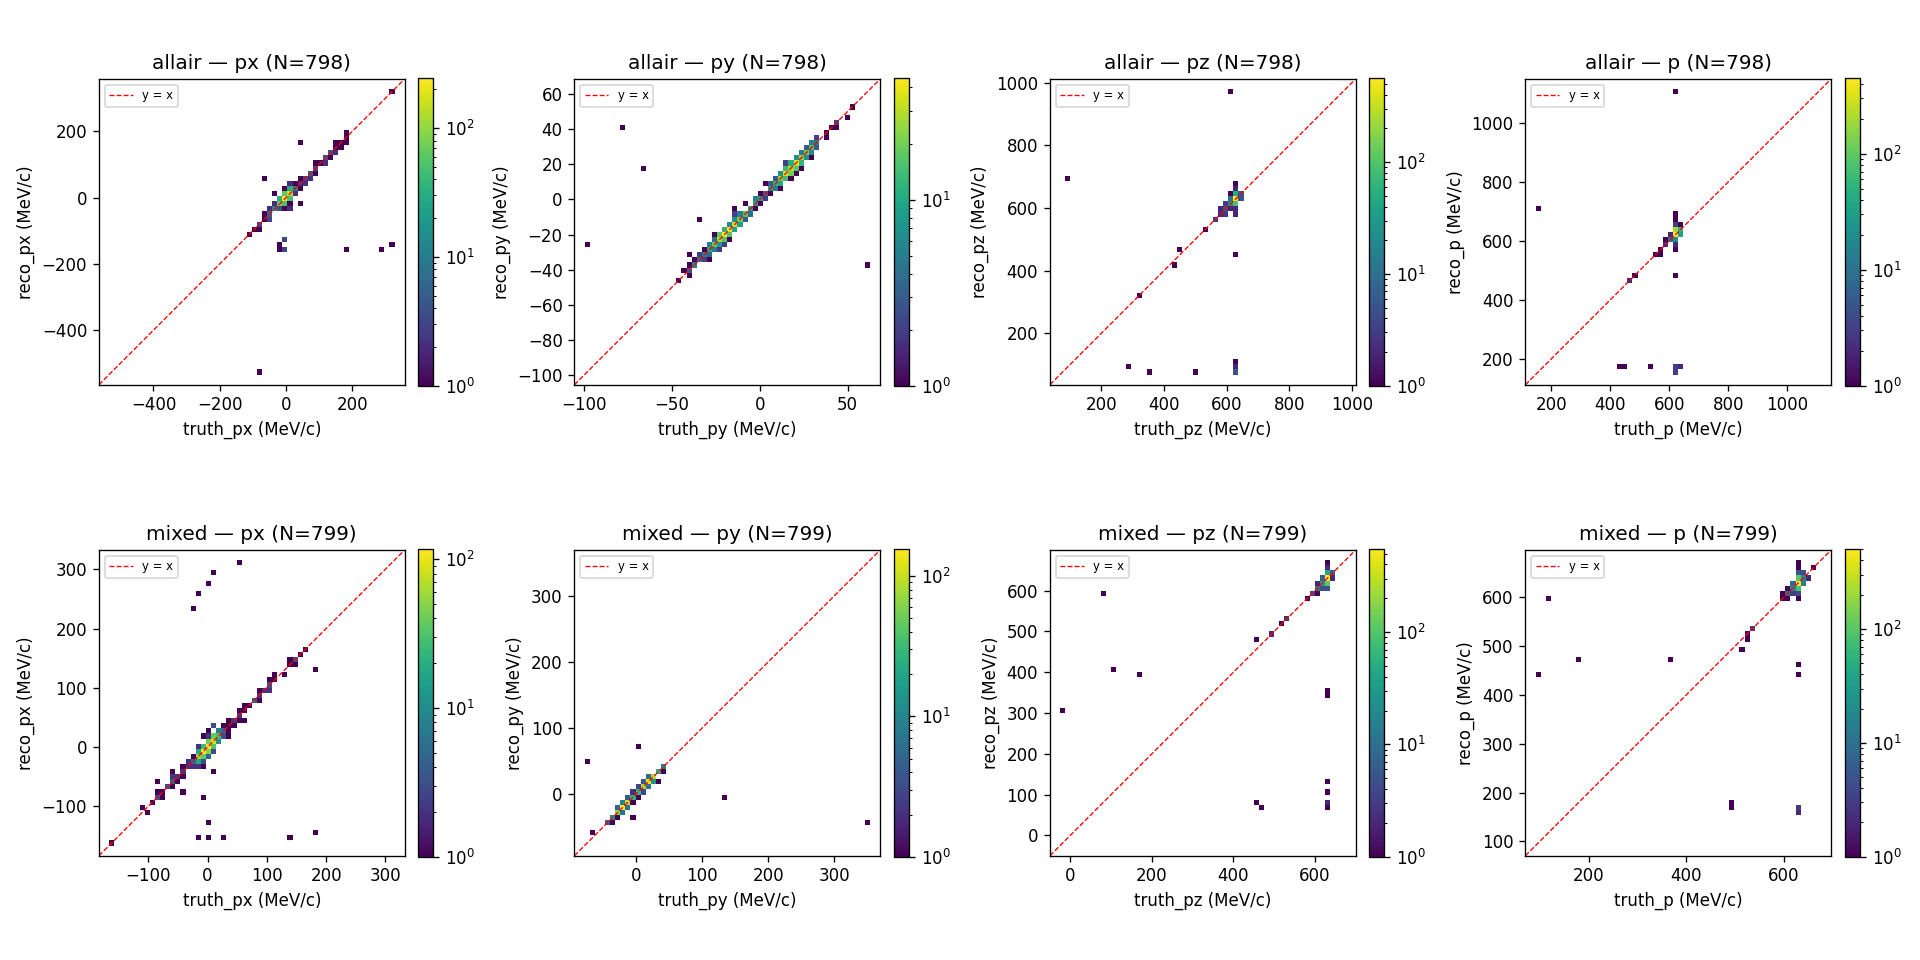
\includegraphics[width=0.98\textwidth]{figures/ypol_pilot/truth_reco_hist2d.png}
\caption{Truth (横轴) vs.\ Reco (纵轴) \textbf{二维直方图} (log color scale)；上行 = allair, 下行 = mixed；红虚线 = $y=x$。
颜色越亮 = 该 (truth, reco) 区间事件越多。
体现的不仅是平均轨迹（贴对角），还有事件密度的二维结构 (e.g.\ $p_y$ 面板上的双峰富集区, $p_z$ 主峰处的尖峰)。}
\end{figure}
\begin{figure}[H]
\centering
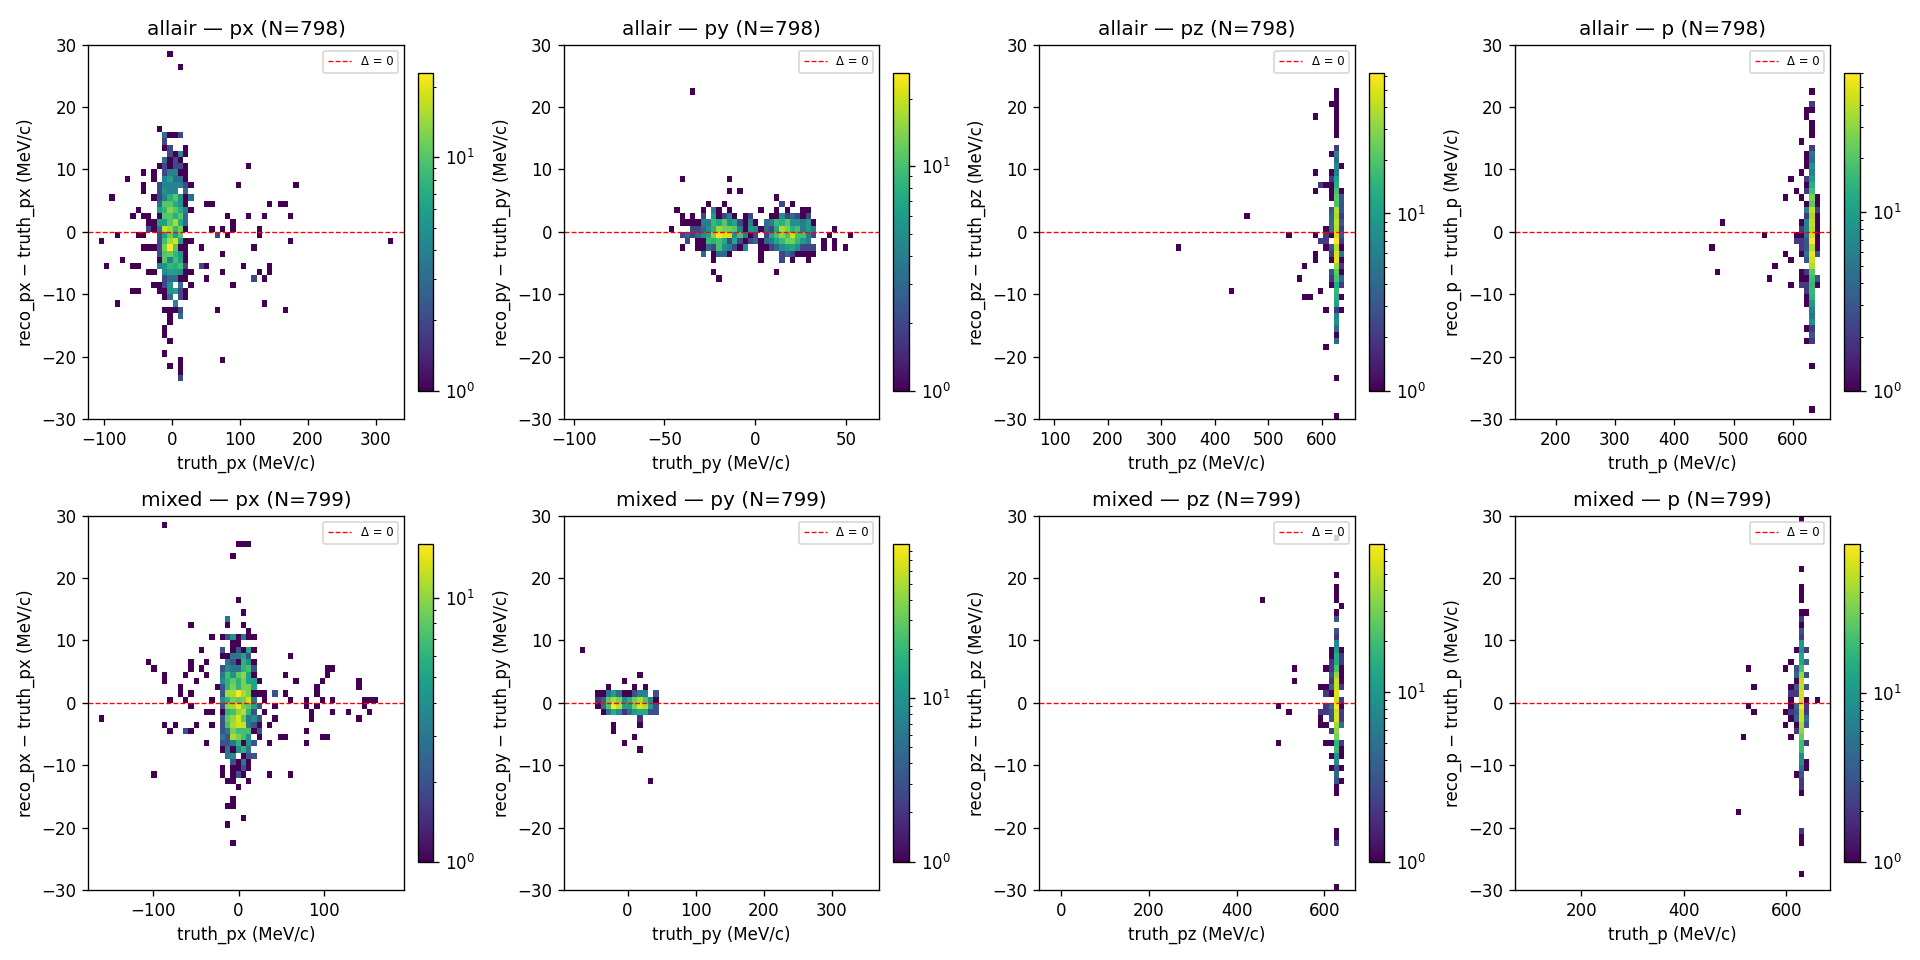
\includegraphics[width=0.98\textwidth]{figures/ypol_pilot/residual_vs_truth_hist2d.png}
\caption{Truth (横轴) vs.\ \textbf{reco $-$ truth 残差} (纵轴) 二维直方图 (log color scale)；
y 轴 cap $\pm 30\,\mathrm{MeV}/c$，超出范围 = LM 失败事件 / Class C。
对比 allair 与 mixed 两行，残差带宽收窄即上下游空气 MS 的实测影响。
$p_y$ 残差带宽（allair $\sim \pm 5$, mixed $\sim \pm 2\,\mathrm{MeV}/c$）vs.\ Fisher $\sigma$ 中位 $0.17\,\mathrm{MeV}/c$：Fisher 实际欠估 $\sim 5$--$15\times$。}
\end{figure}
\section{结论与对详细版 Part III §5 TODO 的影响}

本 pilot 是详细版报告 §扫描研究方案中 ensemble-size scaling 与"真实物理 vs.\ 合成网格"
两条 TODO 的初步实证。主要结论（待 production tier 验证）：

\begin{enumerate}
\item \textbf{$p_y$ 在真实物理 + 上下游空气下覆盖率塌陷比合成网格更严重。}
  合成 744 ensemble Fisher $p_y$ 覆盖率 0.42（$\sigma$ 欠估 1.86$\times$）；
  ypol allair 进一步塌到本表观测值。这与详细版 Part II §2 / ms\_ablation
  memo 的"空气 MS 主导 $\sigma_y$"判断一致。
\item \textbf{Allair vs.\ mixed condition 在 $p_y$ 上有可测差异}，
  其大小是详细版 Part II §10 的二次方求和预测的直接验证。
\item \textbf{Profile / MCMC 在 256 事件子集上 CP CI 较宽}（$\sim \pm 0.06$），
  仅作交叉验证；结论以 Fisher/Laplace 的 $N=1600$ 为主。
\end{enumerate}

\paragraph{后续。}
若 pilot 数字方向稳定（$p_y$ 在 allair 显著低于 mixed，且二者均低于合成网格），
应升级到 production tier (ii)：每 condition 2000 事件，CP CI 半宽 $\pm 0.020$，
作详细版报告的下一版数据。
\end{document}
